\model{Memory Diagrams}

The following diagrams are based on the example code from \ref{model1.tex}.

\vspace{1em}

\textbf{Array of ints:}
\\[1ex]
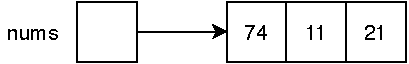
\includegraphics[scale=0.95]{array.pdf}

\vspace{1em}

\textbf{ArrayList of Integers:}
\\[1ex]
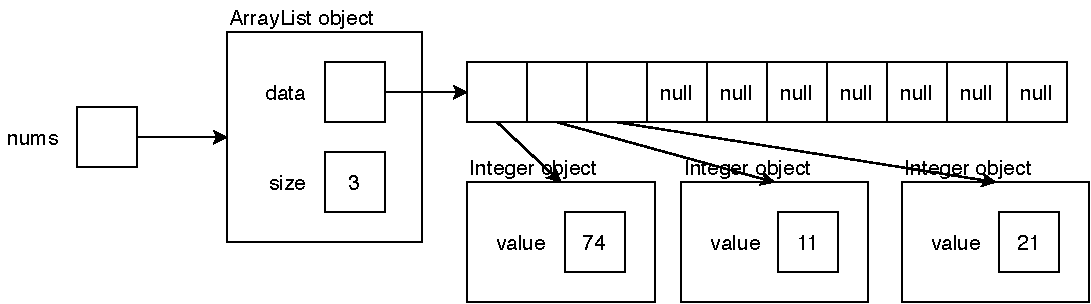
\includegraphics[scale=0.95]{alist.pdf}


\quest{10 min}


\Q What is the \java{length} of the array inside of the ArrayList? \ans[3em]{10}


\Q How are the contents of the \java{data} array different from the array of ints?

\begin{answer}[3em]
The \jans{data} array is storing references to \java{Integer} objects, each of which wraps an \jans{int} value.
The array of ints simply stores the values directly.
\end{answer}


%\Q Based on the diagrams, what is the difference between an \java{int} and an \java{Integer}?
%
%\begin{answer}[3em]
%An \jans{int} is a primitive value that can be stored directly.
%\jans{Integer} is a wrapper class; its value is ``wrapped'' inside of an object.
%\end{answer}


\Q What happens when a fourth element is added to the ArrayList?

\begin{answer}[3em]
(1) An Integer object is created,
(2) it's placed in the next available position of the array,
and (3) the size attribute is incremented.
\end{answer}


\Q \label{key2}
Explain how an ArrayList can ``grow'' when adding new elements.

\begin{answer}[3em]
New elements can be stored in available slots at the end of the array.
If the data array itself is full, then a larger array can be created.
\end{answer}


\Q Why do ArrayLists require so much more memory than arrays?

\begin{answer}
There is a lot of overhead.
Each individual value needs to be wrapped inside of an object.
And the array itself will likely have unused elements at the end.
\end{answer}
